%%%%%%%%%%%%%%%%%%%%%%%%%%%%%%%%%%%%%%%%%%%%%%%%%%%%%%%%%%%%%%%%%%
\section{Introduction}\label{intro}

Multiobjective Optimization Problem have $m$ multiple objective functions that must be optimized simultaneously.

Maximize$^1$ $F(x) = (f_1(x), f_2(x), ..., f_m(x))$,

subject to $x$ in $\Omega$.

- $F(x)$ objective functions;
- $f_i$ is the i-th objective to be maximized;
- $x$ is the decision vector;
- $\Omega$ is the decision space.

\footnotesize $^1$ All definitions are for maximization. Following inequalities should be reversed if the goal is to minimize.

 Many real-world scientific and engineering are MOP.
 Water quality control, Groundwater pollution re-mediation, Design of marine vehicles~\cite{coello2007evolutionary}.
 Petrol extraction.
 Hard problems: to balance the interests of the multi-objective as a whole is hard. 



Objectives may be conflicting
- The goal is to find good trade-off.

- Set of solutions.

Set of *optimum solutions* - Pareto set.

- Non-dominated solutions: no single solution provides a better trade-off in all objectives.

\begin{figure*}[!t]
\centering
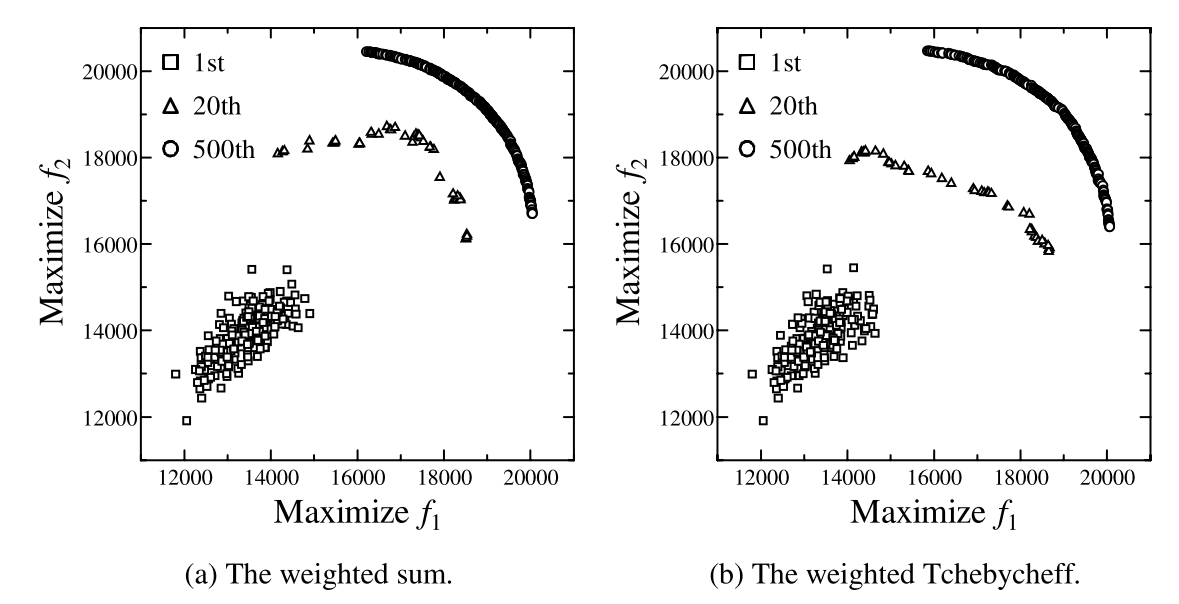
\includegraphics[width=\textwidth]{images/pareto_front_diff_scalarizins_f.png}
\caption{Pareto Set - \cite{ishibuchi2009adaptation} }.
\end{figure*}


1Let $u = (u_1, ..., u_m)$ and $v = (v_1, ..., v_m)$ vectors in $\Omega$ (the decision space).
- $\forall i:u$ dominates $v$ if $f_i(u) \leq f_i(v)$ and $\exists j:f_j(u) < f_j(v)$.
- u dominates v, v is dominated by u, u is better that v.

 A point $x^*$ in $\Omega$  is called *Pareto Optimal* if no other point dominates $x^*$. 


%TODO: This needs to be changed
\begin{figure*}[!t]
\centering
```{r fig.width=3, fig.height=15,echo=FALSE}
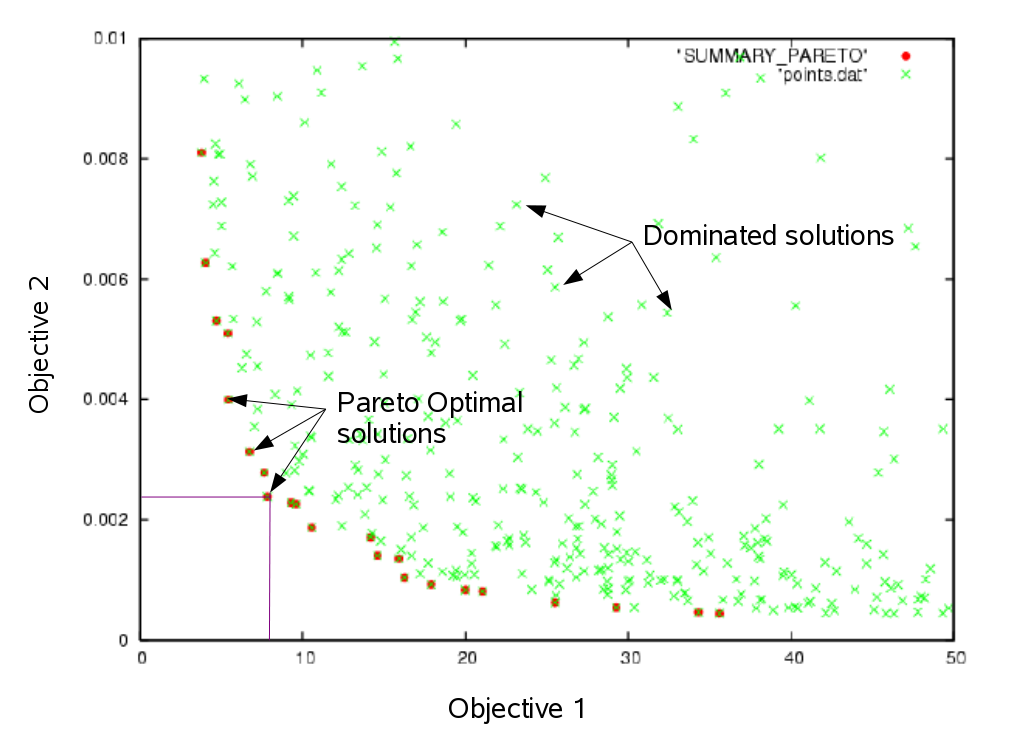
\includegraphics[width=\textwidth]{images/pareto_dominated.png}
%\caption{Pareto Front - From: http://www.cenaero.be/Page.asp?docid=27103&langue=EN}
\end{figure*}

The set of all Pareto Optimal is called the Pareto Set. 

$P^\ast$ = $\{x \in \Omega: \nexists$ y $\in \Omega$ and $F(y) \leq F(x)\}$

 Pareto Front is the image of the Pareto Set in the objective space.
 PF = {$F(x) = (f_i(x), ..., f_m(x)): x \in P^*$}

